\documentclass{template}
\usepackage{graphicx}
\usepackage{subcaption}
\usepackage{algorithm}
\usepackage{algorithmic}
\usepackage{balance}  % for  \balance command ON LAST PAGE  (only there!)
\usepackage{hyperref}


\begin{document}

% ****************** TITLE ****************************************

\title{Worker Recommendation for Q\&A Services}
%\subtitle{[Extended Abstract]
%\titlenote{A full version of this paper is available as\textit{Author's Guide to Preparing ACM SIG Proceedings Using \LaTeX$2_\epsilon$\ and BibTeX} at \texttt{www.acm.org/eaddress.htm}}}

% ****************** AUTHORS **************************************

\numberofauthors{3}
\author{
% 1st. author
\alignauthor
Farbod Shahinfar\\
       \affaddr{Iran University of Science and Technology}\\
% 2nd. author
\alignauthor
Vahid Mohseni\\
       \affaddr{Iran University of Science and Technology}\\
% 3rd. author
\alignauthor
Ehsan Seyed Ali Akbar \\
       \affaddr{Iran University of Science and Technology}\\
}

\maketitle

\begin{abstract}
\label{abstract}
            Worker Recommendation is the core function of Q\&A services 
            such as Qoura and Stack Exchange. 
            Specifically, given a set of tasks to be solved, 
            Worker Recommendation system recommends each
            task to a certain group of workers whom are expected to
            write correct and well writen answers for given task 
            in a short priode of time.

            To address this problem we propose two algorithms. In both
            of these proposed algorithms a way of measuring the relevance of
            a worker to a problem is defined. This measurment is used\
            for recommending a user \(u_i\) for solving a given problem 
            \(p_j\). In the end the top-\(k\) relevant workers are 
            recommended by the system.

            In the algorithm which is discussed first, the idea of
            recommending the worker who is more associated with the tags 
            of question is formulated with a distance function. The lesser
            the distance is the better to recommend the user.

            In the second algorithm, a graph based approch is
            used for modeling the problem in a
            fromal language and suggesting a proper set of
            workers for problem \(p_j\) as an answer.
           
            At the end of this paper both proposed methods are evaluated
            on the data gathered from StackOverFlow question and answer 
            website.
\end{abstract}


\section{Introduction}
\label{sec:intro}
Crowd sourcing is a mean of distributing the process of solving problems.
It is also thought of as a bussiness production model. In this paradaigm,
tasks are distributed among others to be done. This distribution of tasks
should preformed in way that results in less cost for the bussiness. This
cost, depending on the problem and company, may be time, money or other factors
of interest.

A crowd sourcing process involes two groups of users, requesters and workers. 
A requester propose a new task to the system. One or more workers decide to work
on an available task in the system. They choose a task based on their experties and interests. 
The solutions produced for a task are submitted to the requester for evaluation and validation.
The activity history of both requester and worker is recorded for further recommendations.

This process will be efficient only if right tasks are done by appropiate workers.
Moreover, there is no subset of workers to be called appropiate for all tasks
in the system. That is each worker is suitable for certain types of tasks.

For huge bussiness, those with large set of workers and requesters, the rate at
which a new problem is introduced to the system is fairly high. As a result of this
phenomenon, each worker only notices a small subset of tasks.

To help the process of finding a proper task, this paper elaborates a system
to recommend a set of workers for a proposed task. To be more specific during the
paper we have considered the case of Q\&A crowd source system in which tasks are
problems to be answered.

The rest of the paper is structured in the following manner.
Section \ref{sec:prblm-def} defines the problem being examined in this 
paper in a formal language. Section \ref{sec:algo-one} suggests the first algorithm.
Algorithm two is discussed in \ref{sec:algo-two}. 
Section \ref{sec:eval} presents evaluation of our works. 
Section \ref{sec:f-work} and \ref{sec:conclusion} are future work and conclusion respectively.

The implemented algorithms and dataset used for this paper is available online
\footnote{Github repository: \url{https://github.com/vahidmohsseni/rmcourse-recommender}}.


\section{Problem Definition}
\label{sec:prblm-def}
In this paper we focus on presenting an efficient solution for recommending
a set of workers in order to produce proper answers for a set of questions.
The formal definition of this problem is as follows.

Given a set of problems \(P = \{ p_1, p_2, ..., p_n \} \), a set of tags
\(T = \{ t_1, t_2, ..., t_k\} \),
and a set of workers \(W = \{w_1, w_2, ..., w_m \} \) our goal is to 
find a proper subset of workers \(W'  \subseteq W\) for each
problem \( p_j \in P \) which satisfies the conditions of having \(|W'| = k \) and knowing that 
each worker \(w \in W'\) has abilities relevant to the problem \(p_j\).

\section{Algorithm one}
\label{sec:algo-one}
For solving the problem defined in section \ref{sec:prblm-def}, in this part of the paper,
an algorithm is proposed which will prodouce a proper answer. 

The intuition behind this algorithm is to identify an approach for measuring closeness between 
a worker and a given problem. Furthermore this measure of relevance is used to discover workers
who are more related to the given problem. It is supposed that a worker who is considered close
the probelm is enthusiasm of the problem topic and would be able to produce a valid answer for it.
We tried to keep this algorithm as naive as possible. So, the proposed algorithm is simple to trace 
and debug and we are sure that this algorithm is pretty correct and is trustable in results. 

In the continue the algorithm is
examined and its complexity, from both time and memory aspect, is analyzed.

\subsection{Description}
In this algorithm, first, distance of each each worker \((w_i \in W)\) is calculated
from all problems in the given problem set \((\forall p_j \in P)\). Afterward, for each
problem, the top-\(k\) workeres who have the least distances to the problem are chosen. 

Distance between a worker and a problem is defined as formula \ref{f:dist}.

\begin{equation}
 dist(w_i, p_j) = 1 - {{|\{t | t \in Tag(w_i) \cap Tag(p_j)\}| \over {|Tag(p_j)|}}}
 \label{f:dist}
\end{equation}

Algorithm \ref{algo:algorithm1} demonstrates this algorithm with its details.

\begin{algorithm}
        \caption{This is the first algorithm}
        \label{algo:algorithm1}
        \begin{algorithmic}[1]
                \REQUIRE 
                \(W\): set of workers, \(P\): a set of problems,
                \(k\): an integer and \(k \le \lVert W \rVert\)
                \ENSURE 
                \(result\): an array of \(W'_j\) which are subset of \(W\) and \(\lVert W'\rVert = k\)

                \STATE \(result[\lVert P \rVert] \leftarrow \) a new array
                \FOR {\(j = 1\) \TO \(\lVert P \rVert\)}
                        \STATE \(d[\lVert W \rVert] \leftarrow \) a new linked-list
                        \FOR{\(i = 1\) \TO \(\lVert W \rVert\)}
                                \STATE
                                \(d_i \leftarrow dist(w_i, p_j)\) 
                        \ENDFOR
                        \STATE \(W' \leftarrow\) a new set
                        \FOR {\(i = 1\) \TO \(k\)}
                                \STATE
                                \(best\_index \leftarrow argmin(d)\)
                                \STATE
                                \(d.remove(best\_index)\)
                                \STATE
                                \(W'.add(W_i)\)
                        \ENDFOR
                        \STATE \(result_i \leftarrow W'\)
                \ENDFOR
                \STATE return \(result\)
        \end{algorithmic}
\end{algorithm}

\subsection{Complexity analysis}
The algorithm is comprised of a loop wich is repeated \(\lVert P \rVert\) times.
By the product rule it is known that the total time complexity of the algorithm will
be \(\lVert P \rVert \times \theta(\) time complexity of loop body \()\).

The body of the main loop is composed of two other loops and some statements.
% The time of each statement is considered constant and neglectable.
The loop from line 4 to 6 is repeated \(\lVert W \rVert\) times and in each iteration the distance is calculated.
next loop is repeated \(k\) times and in each repetition it search for the minimum value in an array of
size \(\lVert W \rVert\). As a result each iteration will cost \(\lVert W \rVert\) operations, thus, time
complexity of this loop is computed as \(O(\lVert W \rVert\ \times k \).

In total the time complexity of this algroithm, is \(O(\lVert P \rVert \times \lVert W \rVert\ \times k) \).
In the given term, the \(\lVert P \rVert\) is the number of problems a set of workers should be searched for.
The \(\lVert W \rVert\) is the total number of workers available and \(k\) is the number of workers should be
recommended for each problem.

The space complexity of this algorithm is \(O(\lVert P \rVert \times k + \lVert W \rVert)\).

\section{Algorithm two}
\label{sec:algo-two}
Although algorithm one produces correct answers, the time complexity of it, is a concern in a real-world,
practical system. The number of workers of a Q\&A service is much greater than the available tags and for
each problem only a small subset of \(W\) has meaning full distance value. In other words our distance
array for each problem is very sparse. Concluding from this observation, if an approach for pointing out 
the relevant group of workers for a given problem is used for filtering the workeres the time complexity
would be decreased. The result of this decrease in time complexity is proportional to the complexity of 
the filtering approach.
Algorithm two in contrast with algorithm one uses a structured body to solve the problem. This structure 
helps the algorithm two in efficiency which is obvious as mentioned in the next sections.

\subsection{Description}
For improving the time complexity of algorithm one, this algorithm first choses a subset of \(W\).
To achieve this goal a bipartite graph is created once in pre-processing phase, before the system
starts to search for the answers. Then using this data structure the search for a subset of \(W\) is 
perform.

\begin{figure}
    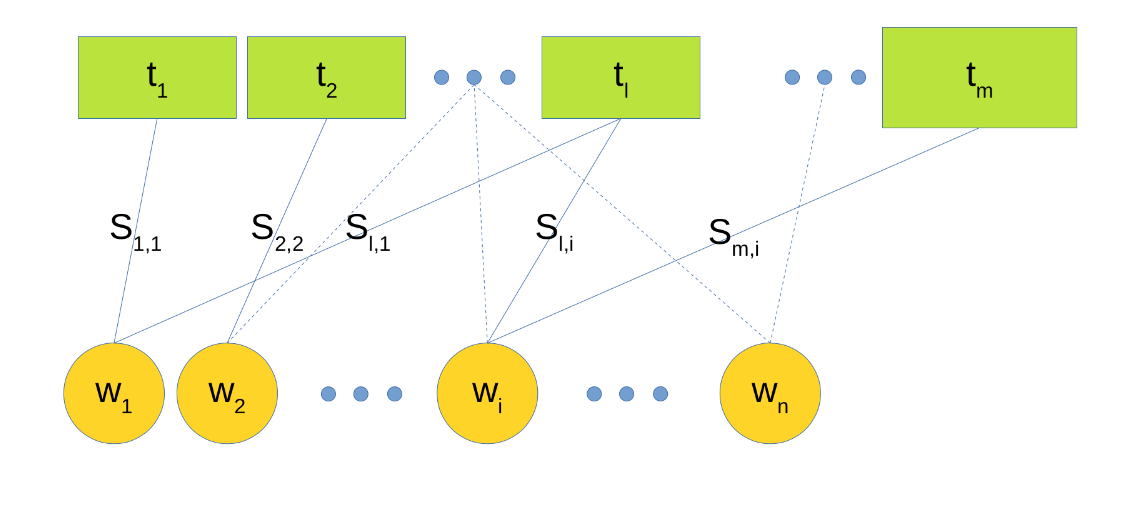
\includegraphics[width=\linewidth]{./images/bpg.png}
    \caption{Structure of a bipartite speciality graph}
    \label{fig:bpg}
\end{figure}

The bipartite graph considered for this algorithm is called speciality graph and
has two groups of nodes. A group of nodes represent available tags in the system
and the other group consist of nodes representing workers. Each worker
who happen to be known to have experties related to a tag, is connected to the corresponding node of that
tag. Moreover this graph is weighted. Each edge connecting a tag \(t_l\) 
to a worker \(w_i\) has a value \(S_{l,i}\) representing the score the worker has gained through 
solving problems of the same tag before. Figure \ref{fig:bpg} shows the general structure of this
graph.

After forming this bipartite graph, the process of choosing top-\(k\) worker for each problem is as follows.
The node corresponding to each tag of the given problem is probbed. For a tag \(t_k\) the workers associated with it is added to a hashmap named score\_table. 
The score value of each chosen worker is aggregated in the score\_table. After creating the score table
the top-\(k\) workers having the highest aggregated score are added to \(W'\). \(W'\) is the set containing
our recommended workers.

Psuedocode in algorithm \ref{algo:algorithm2} depicts the approach described in this section.

\begin{algorithm}
    \caption{This is the second algorithm}
    \label{algo:algorithm2}
    \begin{algorithmic}[1]
        \REQUIRE 
        \(W\): set of workers, \(P\): a set of problems,
        \(k\): an integer and \(k \le \lVert W \rVert\)
        \ENSURE 
        \(result\): an array of \(W'_j\) which are subset of \(W\) and \(\lVert W'\rVert = k\)
        
        \STATE result \(\leftarrow\) new linked-list
        \STATE {specialty\_graph \(\leftarrow\) create\_bipartite\_graph()}
        \FORALL {\(p_j\) in \(P\)}
            \STATE score\_table \(\leftarrow\) a new hashtable
            \FORALL {\(t_l\) in \(Tag(p_j)\)}
                \FORALL {\(w_i\) in specialty\_graph[\(t_l\)]}
                    \STATE worker\_score \(\leftarrow\) specialty\_graph[\(t_l\)][\(w_i\)]
                    \STATE score\_table[\(w_i\)] \(\leftarrow\) score\_table[\(w_i\)] + worker\_score
                \ENDFOR
            \ENDFOR
            \(W' \leftarrow \) a new set
            \FOR {i\(=1\) \TO \(k\)}
                \STATE worker \(\leftarrow argmax(\) score\_table \()\)
                \STATE \(W'\).add(worker)
                \STATE score\_table.remove(worker)
            \ENDFOR
            \STATE result.add(\(W'\))
        \ENDFOR
        \STATE return result
    \end{algorithmic}
\end{algorithm}

\subsection{Complexity analysis}
Time complexity for algorithm two is 
\(O(\lVert P \rVert \times k \times (\)number of workers having one of the problem's tag)\()\).
At the worst case, in which all workers registered in the system have a connection with a tag \(t_l\),
this time complexity will be the same as the algorithm one. But as it was mentioned, because of the 
sparsity of relations between a worker and a tag, the score associated between \(t_l\) and all
workers is zero for majority of cases. As a result, the time complexity is decreased, hence, the 
algorithm two will produce answers with more efficiency.

In contrast to time complexity, space complexity of this alogrithm is the same as the algorithm one.
The specialty tree has data related to all workers so it takes space of \(O(\lVert W \rVert)\). 
Moreover the space required by the algorithm two is
\(O(\lVert P \rVert \times k + (\)number of workers having one of the problem's tag)\()\).

Viewing all aspects together, algorithm two suggests a more efficient approach for
solving the problem specified in section \ref{sec:prblm-def}.

\section{Evaluation}
\label{sec:eval}
\subsection{Data Collection}
The evaluation of this work has been carried out on data gathered from StackOverFlow website.
This data was collected using a crawler script which was used to extract data about problems
and users. The gathered data is comprised of problems id and their correlated tags and users id along
with all the tags a user has been associated with. All of the tags related to a user has a socre value.
These data are stored in a sqlite file in order to be accessed easily.

\subsection{Results}
As it is shown in figure \ref{fig:latency_eval}, the time needed for algorithm two to prepare 
an answer is reduced to less than one third of the algorithm one.

The values presented in figure \ref{fig:latency_eval} are average of latencies measured during testing.
The problems from dataset was splitted to different sets and along with the set of all users where 
given to each algorithm. The \(k\) was set to 5 in all the test.

\begin{figure}
    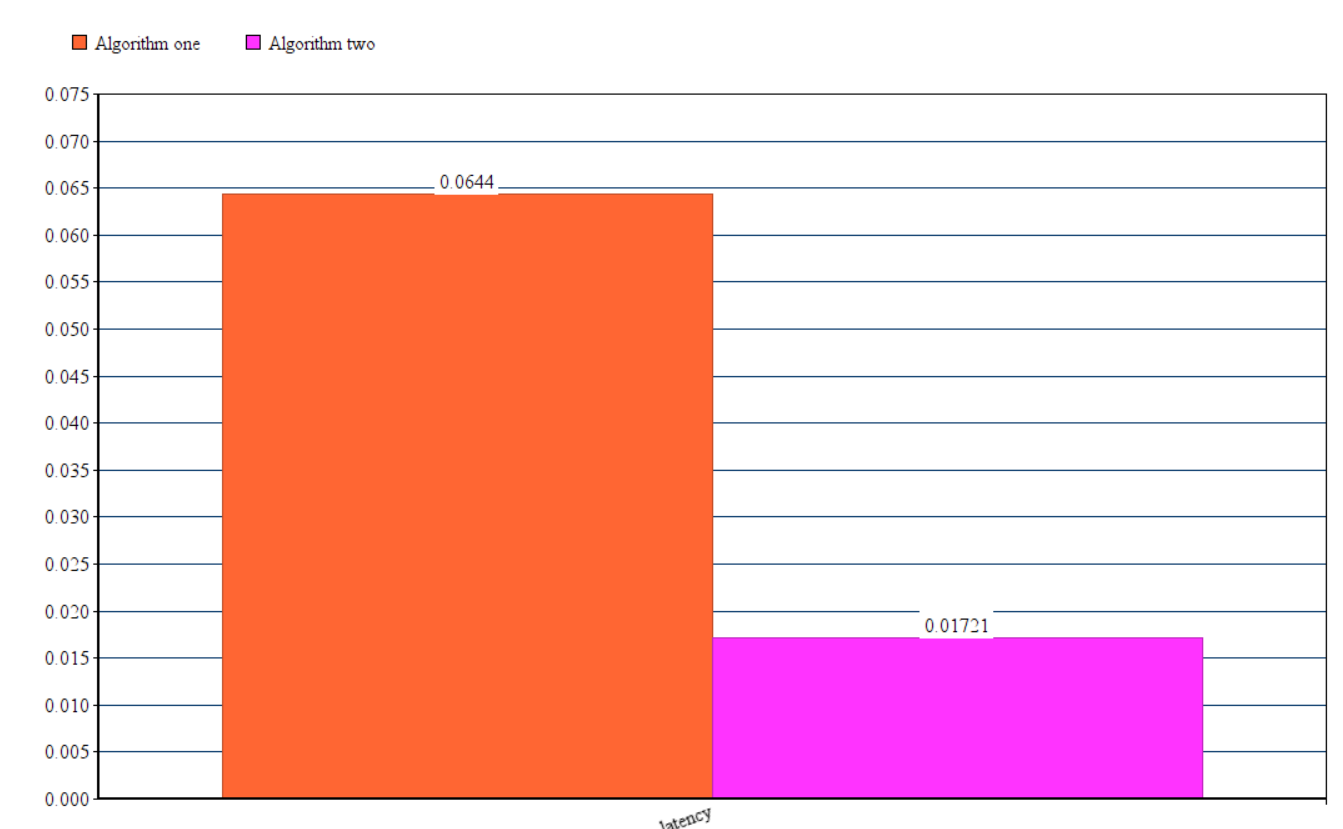
\includegraphics[width=\linewidth]{./images/latency_eval.png}
    \caption{Comparison of latency of each algorithm}
    \label{fig:latency_eval}
\end{figure}

The Time complexity of both algorithm suggests that they scale linearly with respect to \(k\) parameter.
The figure \ref{fig:k-comparison} confirms that both algorithms have linear time complexity with regard
to \(k\).

\begin{figure}
    %\begin{subfigure}{0.9\linewidth}
    %    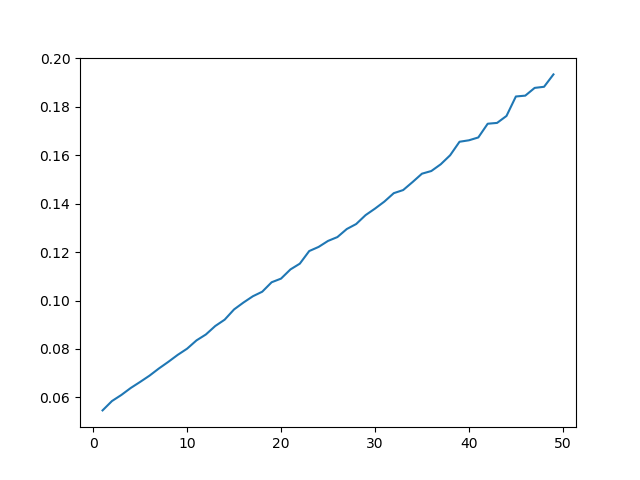
\includegraphics[width=\linewidth]{./images/algo1_diff_k.png}
    %    \caption{Algorithm one}
    %\end{subfigure}
    %\begin{subfigure}{0.9\linewidth}
    %    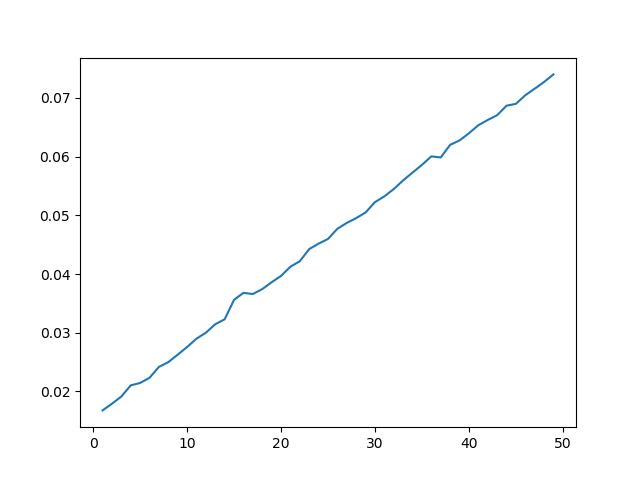
\includegraphics[width=\linewidth]{./images/algo2_diff_k.png}
    %    \caption{Algorithm two}
    %\end{subfigure}
    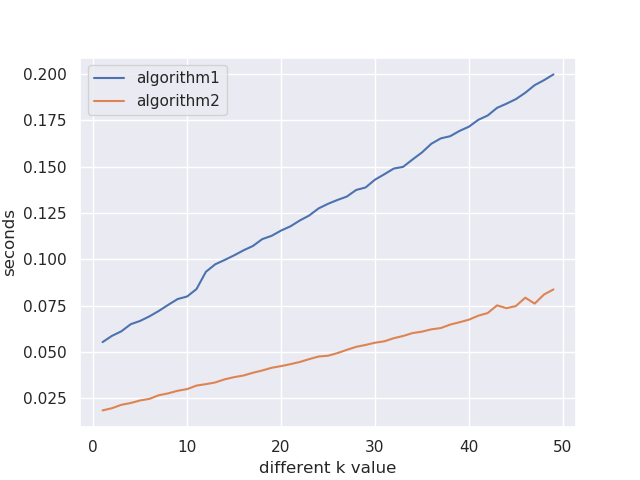
\includegraphics[width=\linewidth]{./images/algo1_algo2_diff_k_sns.png}
    \caption{Clock time duration with different \(k\) values for problem sets of size 50}
    \label{fig:k-comparison}
\end{figure} 


Both algorithms are tested on different size of problem set (\(\lVert P \rVert\)). The result
of the experiments are shown in figure \ref{fig:p-comparison}. It can be concluded that both 
algorithms are linear with respect to the size of problem set. This conclusion complies with
statements in sections \ref{sec:algo-one} and \ref{sec:algo-two}.

\begin{figure}
    % \begin{subfigure}{0.9\linewidth}
    %    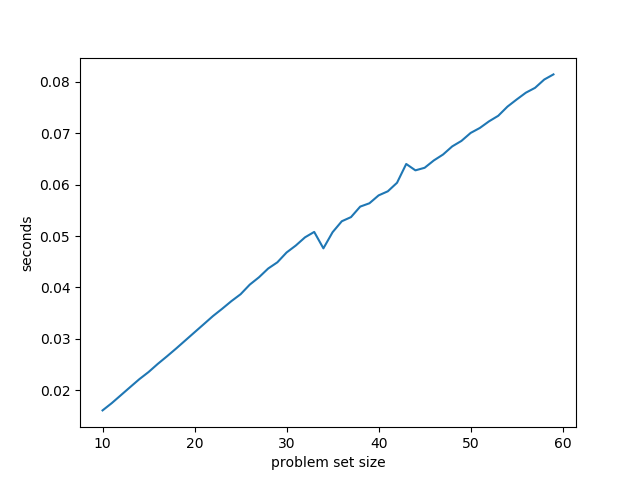
\includegraphics[width=\linewidth]{./images/algo1_diff_p.png}
    %    \caption{Algorithm one}
    %\end{subfigure}
    %\begin{subfigure}{0.9\linewidth}
    %    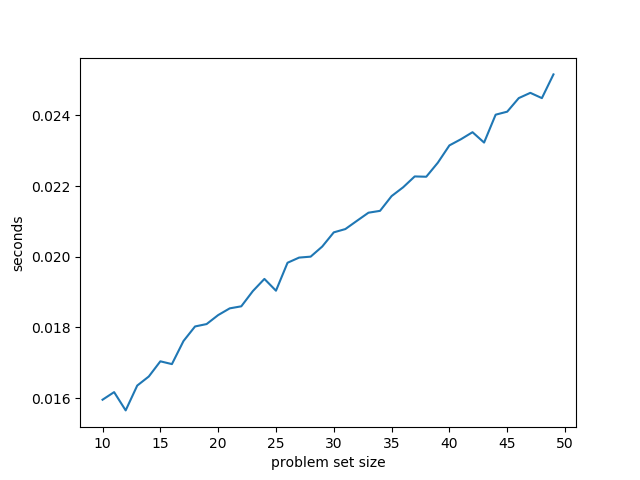
\includegraphics[width=\linewidth]{./images/algo2_diff_p.png}
    %    \caption{Algorithm two}
    %\end{subfigure}
    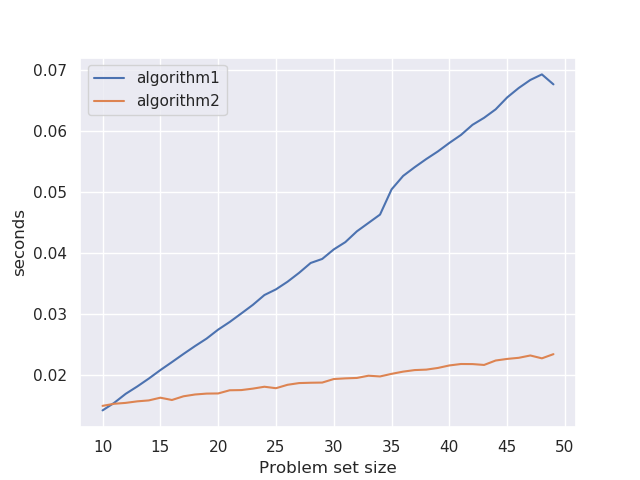
\includegraphics[width=\linewidth]{./images/algo1_algo2_diff_p_sns.png}
    \caption{Clock time duration with different \(\lVert P \rVert\) and \(k=5\)}
    \label{fig:p-comparison}
\end{figure}


\section{Future Works}
\label{sec:f-work}
In future works, we consider examining the effectiveness of our method. We believe algorithm 
two is more effective than the algorithm one but we do not have such a mechanism to evaluate this 
impression yet. Also, we are thinking about new intelligent methods such as machine learning 
techniques for solving this problem and compare them with these algorithms propused in this paper. 


\section{Conclusion}
\label{sec:conclusion}
Crowd sourcing is a distributed approach in solving problems. It aims to reduce cost.
For this system to perform efficiently, it is crucial to have a recommendation system
to offer tasks to relevant workers.
In this paper two algorithms are proposed for finding a subset of workers \(W'\) who
are relevant to a given problem \(p_j\). Both of these algorithms are analysed carefully.
At the end these two algorithms are evaluated on a dataset gathered from StackOverFlow 
Q\&A service.

\end{document}
